
\documentclass[preprint,12pt, authoryear]{elsarticle}

%% Use the option review to obtain double line spacing
%% \documentclass[preprint,review,12pt]{elsarticle}

%% Use the options 1p,twocolumn; 3p; 3p,twocolumn; 5p; or 5p,twocolumn
%% for a journal layout:
%% \documentclass[final,1p,times]{elsarticle}
%% \documentclass[final,1p,times,twocolumn]{elsarticle}
%% \documentclass[final,3p,times]{elsarticle}
%% \documentclass[final,3p,times,twocolumn]{elsarticle}
%% \documentclass[final,5p,times]{elsarticle}
%% \documentclass[final,5p,times,twocolumn]{elsarticle}


\setlength\parskip{\baselineskip}

%% The graphicx package provides the includegraphics command.
\usepackage{graphicx}
%% The amssymb package provides various useful mathematical symbols
\usepackage{amssymb}
%% The amsthm package provides extended theorem environments
%% \usepackage{amsthm}

%to color text
\usepackage{xcolor}

%% The lineno packages adds line numbers. Start line numbering with
%% \begin{linenumbers}, end it with \end{linenumbers}. Or switch it on
%% for the whole article with \linenumbers after \end{frontmatter}.
\usepackage{lineno}

%%to allow for ø and é
\usepackage{inputenc}


\usepackage{hyperref}

\usepackage{csquotes}


%% To include pdfs as appendix
\usepackage{pdfpages}

%% natbib.sty is loaded by default. However, natbib options can be
%% provided with \biboptions{...} command. Following options are
%% valid:

%%   round  -  round parentheses are used (default)
%%   square -  square brackets are used   [option]
%%   curly  -  curly braces are used      {option}
%%   angle  -  angle brackets are used    <option>
%%   semicolon  -  multiple citations separated by semi-colon
%%   colon  - same as semicolon, an earlier confusion
%%   comma  -  separated by comma
%%   numbers-  selects numerical citations
%%   super  -  numerical citations as superscripts
%%   sort   -  sorts multiple citations according to order in ref. list
%%   sort&compress   -  like sort, but also compresses numerical citations
%%   compress - compresses without sorting
%%
%% \biboptions{comma,round}

% \biboptions{}

% remove preprint from foot
\makeatletter
\def\ps@pprintTitle{%
 \let\@oddhead\@empty
 \let\@evenhead\@empty
 \def\@oddfoot{}%
 \let\@evenfoot\@oddfoot}
\makeatother


\newcommand\commenting[1]{\textcolor{red}{\textbf{\underline{#1}}}}

\begin{document}

\begin{frontmatter}

%% Title, authors and addresses

\title{Rat Kid Dog Fight - Ethical Test Survey}

%% use the tnoteref command within \title for footnotes;
%% use the tnotetext command for the associated footnote;
%% use the fnref command within \author or \address for footnotes;
%% use the fntext command for the associated footnote;
%% use the corref command within \author for corresponding author footnotes;
%% use the cortext command for the associated footnote;
%% use the ead command for the email address,
%% and the form \ead[url] for the home page:
%%
%% \title{Title\tnoteref{label1}}
%% \tnotetext[label1]{}
%% \author{Name\corref{cor1}\fnref{label2}}
%% \ead{email address}
%% \ead[url]{home page}
%% \fntext[label2]{}
%% \cortext[cor1]{}
%% \address{Address\fnref{label3}}
%% \fntext[label3]{}


%% use optional labels to link authors explicitly to addresses:
%% \author[label1,label2]{<author name>}
%% \address[label1]{<address>}
%% \address[label2]{<address>}

\author{Carl Johan Hanberg}
\author{Paw H\o vsgaard Laursen}


%%\begin{keyword}
%%Science \sep Publication \sep Complicated
%% keywords here, in the form: keyword \sep keyword

%% MSC codes here, in the form: \MSC code \sep code
%% or \MSC[2008] code \sep code (2000 is the default)

%%\end{keyword}

\end{frontmatter}
\clearpage

\tableofcontents
\clearpage

%% main text

\section{Introduction}
This document is an exempt from the paper \textit{Do Dog Fighters Love Their Dogs?}. It includes only an overview of the testing sessions, and a discussion of and conclusion on the results.

We will produce the mobile dog fighting game ��Rat Kid Dog Fight!��. We will conduct extensive playtests, focusing on the reactions of players in particular game situations.\

The main character in the game will be portrayed as one of the 15.000 homeless children of Mexico City \citep{baverstock}, which tries to break the circle of drug abuse and prostitution, by training stray dogs to battle in the illegal dog fights of the local gangs. This narrative will make dog fighting the only viable option for the character and will be presented as a lesser of two evils, which can help the players justify their own actions. \

The gameplay mechanics will draw similarities to the Pokemon game series \citep{game:pokemon} and other pet management games, where the player is also afforded the option of pitting animals against each other. While we are interested in having minimal player agency in the dog fights, the Pokemon similarities should create the expectancy of player agency \citep{wardrip2009agency}. \

We will determine from the prototype and test data how we can best continue development towards a full-featured mobile game, and if such a game would be best suited for retail distribution or art exhibitions.\

\section{Test Conditions}
\subsection{Method}
To answer our hypotheses we have designed a qualitative play experience test. The procedure of the test includes first a playthrough of the game and then a semi-structured interview. The in-game choices made by the player in the playthrough is recorded as is their body language, statements or other sounds produced while playing.

The test subjects will be asked to participate in one playthrough of the game followed by a semi-structured interview to gather data on that specific play experience. Due to the mature content of the game the targeted test subjects are age 18 or above. To look for trends across genders we aim for gender equality in our sample. Furthermore while recruiting test subjects we look for subjects who has outspoken opinions about dogs, animal rights and/or human rights. The only quantitative data collected is the in-game choices of the game and these are of binary quality at best. 

In-game choices:
In the game you as player has to take several choices regarding the fate of your avatar. \commenting{Avatar or character?? it seems like it depends on the eyes that sees.. INVESTIGATE}

\subsection{Sessions}
Two testing sessions were conducted on the IT University of Copenhagen. The first on the 30th October 2017, the second on the 23rd November 2017. The test procedure followed the same guidelines for both of the tests however a few of the questions were rephrased and the implementation of the game underwent several changes. The changes included correction of spelling in the narrative, more graphical elements depicting the situation of the state of the game and better feedback in the dog fights in the game. These changes will have biased the test results and should be kept in mind when analysing the data.

A playthrough of the game took 10-15 min. depending on the speed of the participant - reading, taking decisions - and the random outcomes of the fights in the game. While playing the participants in-game choices was recorded. Some participants came to an end of the game after the second fight of the game others after the third.
The interview was conducted following af semi-structured questionnaire consisting of 17 predefined questions, participant demographics questions and a small observational sheet to record the actions taken by the participant in the game. Furthermore observations of the participants body language, statements and other kinds of sounds while playing the game was recorded.

\subsection{Results}
In total nine subjects, four male and five female, successfully participated in the test. The youngest being 24 and the oldest 31, average being 27,2 years old. Six of the participants are higher education students, two are film directors and the last participant is educated but unemployed. It is safe to conclude that the participants on average possesses intellectual judgement.

The most important choice of the game is where the player is asked to choose their destiny. Whether they will participate in dog fighting or offer sexual favours to earn money. Six participants chose dog fighting, three chose sexual favours. All but one of the participants made the choice relatively quickly between three to nine seconds. The one exemption spend a minute before choosing dog fighting.

\subsection{Discussion}
In the following paragraph test subjects will be referred to by number 1-9. 

IS DOG FIGHTING THE BETTER ALTERNATIVE?
One of the things we were curious about is whether dog fighting is perceived as a better alternative to prostitution. It is no secret that in our - the designers - mind dog fighting is a better alternative. Our test data indicate that the majority of the participants felt the same way but we cannot ignore the data that resists this notion. A trend in the data reveals that the visual appearance of the man you are to prostitute yourself to has had an impact on the choice. We might also have to question whether the choice is affected by the player's cultural background.

One participant(2) spend a minute making the decision. She was clearly emotionally affected by the game and the choice made her feel uncomfortable. Interestingly she was part of the first test session. In the implementation of the game used for the first session the man to which you can offer sexual favours is not depicted. In the second implementation of the game he is depicted as being very repulsive.  \commenting{Insert picture of man} The fact that he is not depicted in the first test session may have made the choice less unambiguous. This thought is supported by two other participants(7, 9) statements to the question "Why did you pick dog fighting over sexual favours?". They state that the man's uglyness played a role in their decision to pick dog fighting. A fourth participant(8) states that he felt the game wanted him to choose dog fighting over sexual favours. Whether the depiction of the man has had an impact on this can only be speculated but it seems like the new implementation of the game pushes the player more towards picking dog fighting over sexual favours.

Two(1, 6) of the three participants who chose sexual favours over dog fighting stated that they chose sexual favours out of curiosity. Observations of the participants, a male and a female, indicate that they were taking the seriousness of the game lightly and were having fun with it. They seemed to have a satirical distance to the game. The male participant(1) states that he chose the sexual favours because it was more extreme. The female(2) states that her choice may have been biased because she was sitting at a test. Their data indicate that they felt that dog fighting was the moral choice but that they chose sexual favours just to see what would happen in the game. Interestingly the last participant(4) chose sexual favours because she felt that it was the moral choice. Born and raised in Hong-Kong her cultural background is different from the rest of the participants (native Danes). Her reasoning being that no one dies in the sexual favours scenario. She is aware of, and believes that her opinion and choice is different from the other test participants. However she herself states that it is because of her cultural background.

CHARACTER / AVATAR AND DOG
A central question regarding the game design is how emotionally invested the players are in the game. Our goal was to create a play experience that had en emotional impact on the player that goes beyond pure entertainment. We believed that this could be achieved by first creating a gloomy narrative set in a - close to - real environment and by creating affordances that makes the player experience the story as being the protagonist rather than observing.  The participants identification with the depicted protagonist of the game and the participants perceived roles in the game indicates that the participants played the game in different ways. We cannot quantify the participants emotional investment but there are trends in the data that indicate how the players felt while playing the game. The data indicates that the players have different perceptions of the protagonist as an avatar. To some he is a rounded character whos fate the players decide, to others he is a projection of player's self in his reality. To avoid a confusion of the character versus the avatar we will refer to the protagonist as the 'protagonist' in the following paragraph.

The second decision the participants had to make in the game was to give the protagonist a name. Six participants(1, 2, 3, 4, 5, 7) chose to give the protagonist a what we define as a serious name. The serious names are names that resemble the participants real name or is a known nickname of theirs while the non-serious names are not. We speculate that the participants chose a serious name because they want to identify with the protagonist rather than distance themselves from him. While picking a non-serious name is a way to create a humorous distance between yourself and the protagonist in the game. This speculation is partly supported by the data. One of the participants(6) who chose a non-serious name was experiencing the whole game as a satire, she clearly had a humorous distance to the entire play experience. Another participant(9) who chose a non-serious name states that he did not identify with the protagonist and that it was a conscious decision to give the protagonist a non-serious name. However data from three of the participants(1, 4, 7) who chose a serious name indicates that they did not identify with the protagonist. Hence the name to protagonist relationship hypothesis does not seem to apply. Instead choosing a serious name may be an expression of how willing you are to invest emotions in the game.

Interestingly the serious name pattern changes when the participants are asked to give their dog a name. Now only two participants(2, 7) chose to give their dog a serious name. This shift might indicate either that the game has made the participants perceive their role in the game differently or that the participants are trying consciously to distance themself from the either the game or the dog in the game. Participant 5 and 9 states that they chose a funny or distancing name to avoid getting too close to the dog. The data of participant 4 indicate the same trend but is less clear cut. Participants 1, 3 and 8's data indicate that they did not yet feel attached to the dog the moment they had to give it a name. Participant 6 was as explained earlier having a satirical distance to the entire game experience.
Interestingly only two participants(6, 8) chose to leash the dog however both of them expressed that they thought it was the correct option, implying that they were afraid of the consequences if they did not leash it. Participant 1, 2, 3, 7 and 9 express that they believe their relationship with the dog would be improved by not leashing it. Participant 4 and 5 both express that leashing it would have made the dog easier to control, but chose to not leash it. The findings indicate that the name can be perceived as an indication of emotional engagement in the game. Moreover it seems that our implementation did a sub par job at creating the necessary emotional bonding to the dog prior to the naming of it.


CAN WE CREATE UNETHICAL AFFORDANCES, NAMELY DOG FIGHTING, IN A GAME WITHOUT MAKING IT AN UNETHICAL GAME?

To the question "Do you think it was an unethical game?", six participants(1, 2, 3, 4, 7, 9) answered no, two(5, 8) answered yes and one(6) answered that it did not matter as the game is satire. Participant 5 elaborates that he believes the Mexicans will oppose the game, but that in a sense the game is not more unethical than other games. He believes that human fights is more unethical, implying that the while unethical the game can exist under the socially accepted unethical threshold of games. Participant 8 elaborates that the humor in the game makes it very unethical, but that its existence is still justified. Participants 1, 2, 3, 4 & 7 elaborates that the game makes you are aware and puts you in the horrible situation of the game, implying that your actions are justified by the situation you are in. Participant 4 and 7's only real complaint was that they wanted a disclaimer for the blood on the dogs.
When asked if the game was moralising seven participants(1, 2, 3, 5, 6, 8, 9) answered no, one(4) answered yes and the last one(7) was not sure. Participants 1, 2, 3 and 5 elaborates that the game itself does not tell you what is right or wrong. Participant 4 states that the game is trying to hint something. She is not defining what the game is hinting but says the game is made to make you feel bad by dismembering and putting blood on cute dogs. Participant 7 also cannot define what the moral of the game is but that it is hard that the game forces her to downprioritise her dog. 


WILL THE PLAYER BE ABLE TO FEEL EMPATHY FOR THE DOGS, WHILE BEING RELIANT ON THEM FIGHTING?

The participants choice of dog described in their responses to the question "Why did you pick the dog you picked?" are coded as being either a choice based on feelings or rationale. Six participants(2, 3, 4, 5, 6, 7, 9) made a rational decision on their choice of dog. They base their decision on which dog they felt was best capable of fighting. In contrary participant 1 and 8 based their choice of dog on feelings. Participant 1 chose the husky because he thought it was cool but speculate that the boxer might have been more capable of fighting. Participant 8 did not choose the boxer because he was too emotionally attached to it and he wouldn't want to see it suffer. His response raises the question whether the other participants seemingly rationale choices are made on the basis of choosing the dog that would suffer the least. If that is the case then the participants choices are based on feelings in the sense that they choose the dog that will have the least emotional impact on them.



\begin{table}[h]
\centering
\begin{tabular}{l l l}
\hline
\textbf{Destiny} & Sexual favours & Dog fight\\
\hline
Male & 1 & 2 \\
Female & 4 & 2 \\
\hline
\end{tabular}
\caption{Table caption}
\end{table}

A cross reference to table \ref{tab:one}
\begin{table}
\begin{tabular}{|c|c|c|}
\hline 
 This & is & a table \tabularnewline
\hline 
\end{tabular}
\caption{\label{tab:one}The caption of table one}
\end{table}



TO-DO:...
Take the previous written stuff and see if it fits as answers to the three hypotheses. Find more trends in the data. Structure the whole testing paragraph in a better way. At least make subsection titles better. Get more into agency versus avatar versus character and use proper references.
ie. 

Wardrip-Fruin, Noah et al. (2009): "Agency Reconsidered.? Breaking New Ground: Innovation in Games, Play, Practice and Theory. Proceedings of DiGRA 2009, URL: http://www.digra.org/digital-library/publications/agency-reconsidered/

Linderoth, Jonas. (2005): Animated game pieces. Avatars as roles, tools and props. In Aesthetics of Play Conference Proceedings, URL: http://www.aestheticsofplay.org/linderoth.php

Klevjer, Rune (2012): "Enter the Avatar: The Phenomenology of Prosthetic Telepresence in Computer Game?. In The Philosophy of Computer Games (pp. 17-38). Springer Netherlands.






\section{Discussion}
\label{Discussion}
The discussion of the test results will take its starting point in he research questions formulated in section \ref{ProbStat}. 


\textbf{TOPICS:} \
Does loss of agency in fights result in an augmented perception of the game situation being realistic? (p.6 & RQ3)\
Is the seriousness of the player's chosen of name for the protagonist and the dog an expression of their emotional engagement in the game? (p.19 & p23Q6) and what does their rationale behind their choice of dog tell us about it?(p.23) Furthermore is the action of not leashing their dog a signifier of their emotional engagement or does the players actions to this choice raise other questions?(p.23)\
Why does only the participants from session 1 feel responsible for the dogs their dog killed? Are there other signs in the data of session 1 being different than session 2? Why are they different? Why are the results biased. (p. 24 & discussion about man graphics Q3) \
Are there any indications of gender differences in the test data?(p.21)


\textbf{OTHER TOPICS:}\
Validity of test, what was the intention, what could have been done differently?





\textbf{RQ1: Can we create unethical affordances, namely dog fighting, in a game without making it an unethical game?}
The participants responses to Q13 and Q14 indicate that our game is neither perceived as being unethical nor moralising. The trend in the data shows us that the participants bought the premise of the game and felt that the situation you - the protagonist - is placed in justifies your otherwise unethical actions \commenting{sicart ethics maybe}. Unfortunately their responses does not answer our research question in the general sense the question is asked. We know how test participants react to the game after having played it, but we do not have any data on how the common consumer will react to a game like this once it surfaces in public. The game contains enough sensitive subjects to create a solid foundation for public outcry. Even before its release in 2009 \textit{Resident Evil 5} \citep[RE5]{game:re} med massive criticism for its portrayal and dealing with African culture and Africans as zombies \citep{harrer2015black}. Another example from 2015 is when Serious Games had to remove a mini-game, popularly known as "Slave Tetris", in their educational serious game \textit{Playing History 2: Slave Trade}  due to a public outcry \citep{kotaku}. Common to both games is that people defending them claim that the games are subject to misinterpretation by people who have not played them \citep{harrer2015black, kotaku, mtv}. Without going further into the arguments for and against the games it seems like games containing controversial subject matter are subject to superficial interpretations of the games purposes. A hypothesis supported by Deterding's \citeyear{deterding2016mechanic} work showing that the framing of the game plays an important part in the reception of the game.

\blockquote{...Playing History 2 travelled public discourse in the form of a single screenshot of the ?Slave Tetris? level, designed in a child-friendly cartoon look, cutting away the internal critique of the modeled proceedings later in the game. By framing itself as a game for children, it activated a children?s entertainment game frame, which clashed with the serious subject in the audience?s perception.}\citep{deterding2016mechanic}\

Whether our framing of \textit{Rat Kid Dog Fight!} publicly justifies its existence we cannot know. One participant (5) expressed that he believed the Mexicans would oppose the game. The implementation of the game is very much a prototype and its fair to say that the depiction of Mexico City's slum culture is based on loose evidence and gut feelings. The above example of games that fail to frame their purpose should stand as a reminder that we have to carefully analyse and design for the right framing of the game in a future implementation.


\textbf{RQ2:  Will the player be able to feel empathy for the dogs, while being reliant on them fighting?}
The unanimous responses to Q17 ("Do dog fighters love their dogs?") illustrates well that the players had or could imagine having an emotional relation to their fighting dog. However it is hard to find a clear cut answer to whether our test participants felt empathy for their dogs in the game. To try and deduct an answer from the test results we have to broaden our investigation and look for trends that reveal the participants emotional engagement with the game starting with the participants relation to the protagonist of the game. In the paragraph of "Chosen protagonist name" in chapter \ref{ingamedec} we raise the question whether the choice of name for the protagonist is a reflection of the participants emotional engagement with the game. One of the participants (6) who chose a non-serious name was experiencing the whole game as a satire, she clearly had a humorous distance to the entire play experience. Another participant (9) who chose a non-serious name states that he did not identify with the protagonist and that it was a conscious decision to give the protagonist a non-serious name. However data from three of the participants (1, 4, 7) who chose a serious name indicates that they did not identify with the protagonist. The data does not provide a conclusive answer but when correlated with the data of the questions involving the participants dogs it seems like the choice of name for both dog and protagonist is a reflection of how willing the participant is to let herself be emotionally engaged in the game. In contradiction to the chosen protagonist name only two participants chose to give their dog a serious name. As described in the paragraph of "Q6" in chapter \ref{interview} three participants expressed that they chose a non-serious name for their dog to avoid getting too close to it emotionally. This points us in the direction that the participants use the naming of both the dog and the protagonist to adjust their emotional engagement to a level they are comfortable with. We interpret the shift in serious names from 5 (protagonist) to 2 (dog) as a sign of raised emotional engagement over the course of the game. The players choose to give the dogs non-serious names not because it is an expression of their relation to the dog itself but a way of adjusting their emotional engagement so they are less vulnerable for whatever they would meet later in the game. This correlates well with the data of both Q6 and Q7 in chapter \ref{interview}. The participants liked their dogs and they chose not to leash them to avoid damaging their relationship to them. Furthermore the majority of the participants expressed sadness upon the dogs death and a sense of responsibility towards the dog. The discussion presented in this paragraph show that the players try to create a distance to the dogs and the game via non-serious naming of their dog. Upon naming the dog the participants were aware that the dog was going to be used in for dog fighting. Even so they still made decisions that signifies emotional bonding to the dog. Hence we believe the majority of the participants felt empathy for their dog. 



\textbf{RQ3: How does the player feel, when they lose their dogs, while lacking the agency to prevent it?}








IS DOG FIGHTING THE BETTER ALTERNATIVE?
One of the things we were curious about is whether dog fighting is perceived as a better alternative to prostitution. It is no secret that in our - the designers - mind dog fighting is a better alternative. Our test data indicate that the majority of the participants felt the same way but we cannot ignore the data that resists this notion. A trend in the data reveals that the visual appearance of the man you are to prostitute yourself to has had an impact on the choice. We might also have to question whether the choice is affected by the player's cultural background.

One participant(2) spend a minute making the decision. She was clearly emotionally affected by the game and the choice made her feel uncomfortable. Interestingly she was part of the first test session. In the implementation of the game used for the first session the man to which you can offer sexual favours is not depicted. In the second implementation of the game he is depicted as being very repulsive.  \commenting{Insert picture of man} The fact that he is not depicted in the first test session may have made the choice less unambiguous. This thought is supported by two other participants(7, 9) statements to the question "Why did you pick dog fighting over sexual favours?". They state that the man's uglyness played a role in their decision to pick dog fighting. A fourth participant(8) states that he felt the game wanted him to choose dog fighting over sexual favours. Whether the depiction of the man has had an impact on this can only be speculated but it seems like the new implementation of the game pushes the player more towards picking dog fighting over sexual favours.

Two(1, 6) of the three participants who chose sexual favours over dog fighting stated that they chose sexual favours out of curiosity. Observations of the participants, a male and a female, indicate that they were taking the seriousness of the game lightly and were having fun with it. They seemed to have a satirical distance to the game. The male participant(1) states that he chose the sexual favours because it was more extreme. The female(2) states that her choice may have been biased because she was sitting at a test. Their data indicate that they felt that dog fighting was the moral choice but that they chose sexual favours just to see what would happen in the game. Interestingly the last participant(4) chose sexual favours because she felt that it was the moral choice. Born and raised in Hong-Kong her cultural background is different from the rest of the participants (native Danes). Her reasoning being that no one dies in the sexual favours scenario. She is aware of, and believes that her opinion and choice is different from the other test participants. However she herself states that it is because of her cultural background.

CHARACTER / AVATAR AND DOG
A central question regarding the game design is how emotionally invested the players are in the game. Our goal was to create a play experience that had en emotional impact on the player that goes beyond pure entertainment. We believed that this could be achieved by first creating a gloomy narrative set in a - close to - real environment and by creating affordances that makes the player experience the story as being the protagonist rather than observing. The participants identification with the depicted protagonist of the game and the participants perceived roles in the game indicates that the participants played the game in different ways. We cannot quantify the participants emotional engagement but there are trends in the data that indicate how the players felt while playing the game. The data indicates that the players have different perceptions of the protagonist as an avatar. To some he is a rounded character whos fate the players decide, to others he is a projection of player's self in his reality.

The second decision the participants had to make in the game was to give the protagonist a name. Six participants(1, 2, 3, 4, 5, 7) chose to give the protagonist a what we define as a serious name. The serious names are names that resemble the participants real name or is a known nickname of theirs while the non-serious names are not. We speculate that the participants chose a serious name because they want to identify with the protagonist rather than distance themselves from him. While picking a non-serious name is a way to create a humorous distance between yourself and the protagonist in the game. This speculation is partly supported by the data. One of the participants(6) who chose a non-serious name was experiencing the whole game as a satire, she clearly had a humorous distance to the entire play experience. Another participant(9) who chose a non-serious name states that he did not identify with the protagonist and that it was a conscious decision to give the protagonist a non-serious name. However data from three of the participants(1, 4, 7) who chose a serious name indicates that they did not identify with the protagonist. Hence the name to protagonist relationship hypothesis does not seem to apply. Instead choosing a serious name may be an expression of how willing you are to invest emotions in the game.

Interestingly the serious name pattern changes when the participants are asked to give their dog a name. Now only two participants(2, 7) chose to give their dog a serious name. This shift might indicate either that the game has made the participants perceive their role in the game differently or that the participants are trying consciously to distance themself from the either the game or the dog in the game. Participant 5 and 9 states that they chose a funny or distancing name to avoid getting too close to the dog. The data of participant 4 indicate the same trend but is less clear cut. Participants 1, 3 and 8's data indicate that they did not yet feel attached to the dog the moment they had to give it a name. Participant 6 was as explained earlier having a satirical distance to the entire game experience.
Interestingly only two participants(6, 8) chose to leash the dog however both of them expressed that they thought it was the correct option, implying that they were afraid of the consequences if they did not leash it. Participant 1, 2, 3, 7 and 9 express that they believe their relationship with the dog would be improved by not leashing it. Participant 4 and 5 both express that leashing it would have made the dog easier to control, but chose to not leash it. The findings indicate that the name can be perceived as an indication of emotional engagement in the game. Moreover it seems that our implementation did a sub par job at creating the necessary emotional bonding to the dog prior to the naming of it.





TO-DO:...
Take the previous written stuff and see if it fits as answers to the three hypotheses. Find more trends in the data. Structure the whole testing paragraph in a better way. At least make subsection titles better. Get more into agency versus avatar versus character and use proper references.
ie. 

Wardrip-Fruin, Noah et al. (2009): "Agency Reconsidered.? Breaking New Ground: Innovation in Games, Play, Practice and Theory. Proceedings of DiGRA 2009, URL: http://www.digra.org/digital-library/publications/agency-reconsidered/

Linderoth, Jonas. (2005): Animated game pieces. Avatars as roles, tools and props. In Aesthetics of Play Conference Proceedings, URL: http://www.aestheticsofplay.org/linderoth.php

Klevjer, Rune (2012): "Enter the Avatar: The Phenomenology of Prosthetic Telepresence in Computer Game?. In The Philosophy of Computer Games (pp. 17-38). Springer Netherlands.

Harrer, S., & Pichlmair, M. (2015). Black Skin White Guns: Becoming Colonizer in Resident Evil 5.




\section{Conclusion}
%Ethical or not?\
%back story
In our prototype of \textit{Rat Kid Dog Fight!} we tried to allow for the player to participate in dog fights but also to reflect over the concept of dog fighting and the conditions of street kids in Mexico City. We did this by creating a linear experience, where the player was put in the place of a street kid, using both the setting and the choice between two evils as narrative means of justifying the participation in dog fighting.\

%worked - as seen by testers.
We deem this experiment as successful with regards to our testers mostly not viewing the game as unethical. Many of our testers also reflected on the lives of homeless children and the culture of dog fighting describing the experience as unpleasant but educational and thought-provoking.\

%also important not to moralize
It was also our ambition to not create a moralising experience. We did not want the players to feel like they had to act or behave in a certain way for the game to reward and allow them to feel and act towards the dogs as they wanted within the confines of the game. While most testers found the game to not be moralising there were still testers that felt they had to pick specific actions because they were the \textit{correct} ones. \

%Moral or not? General reaction as ethical and not moralizing. Emil thought humour made it unethical. Thora thought of it as a piece of art and hence morality and ethics were not important, just the message.\

%Reaction to no agency. \
We were careful to not arbitrarily reward unethical behavior but simply present the options as a means of survival. We still tried to create some discomfort by creating an illusion of agency in the fights which were meant to be broken. This would hopefully have created an understanding of the impotence of the main character. Unfortunately only one of our testers discovered the lack of agency and that only made him lose interest in the gameplay even though he did understand the mechanic being an allegory of the kid's situation.\ 

%Dilemma of research - blind testing vs. questions before testing.
%	how would we do the test over

We established that it could be possible to create an actual game about dog fighting without it becoming unethical or moralising by default. To develop a game like this we would not include the same amount of humour especially in regards to the Pokemon references. We would not include the illusion of agency but still allow for player superstition, by being able to shout commands during the fight. Instead we would focus on the actual gameplay - the breeding, catching and training of your dogs - and then ultimately dealing with the unlucky loss of your best friend. A game like this could either aim at being released as an art work at an exhibition or as a retail release, as long as it is accurately framed, and the gameplay affordances and marketing reflects it.\

%Implementation and platform for the future game.\ less humour, choise removed, no illusion of agency, but room for superstition and focus on where the agency really is.
No matter the actual implementation, the most important thing is to not remove the \textit{bite} of the game \- not remove its curiosity for man's darker feelings or forgotten creatures, nor its attempt at an artistic expression. While sensibilities might change as the norms of our society does, it is always the responsibility of the artist to push at and test the boundaries of those sensibilities, as well as their legitimacy. \

%% References
%%
%% Following citation commands can be used in the body text:
%% Usage of \cite is as follows:
%%   \citep{key}          ==>>  [#]
%%   \cite[chap. 2]{key} ==>>  [#, chap. 2]
%%   \citet{key}         ==>>  Author [#]

%% References with bibTeX database:

\section*{\refname}
\bibliographystyle{elsarticle-harv}
\bibliography{references}

\


%% Authors are advised to submit their bibtex database files. They are
%% requested to list a bibtex style file in the manuscript if they do
%% not want to use model1-num-names.bst.

%% References without bibTeX database:

% \begin{thebibliography}{00}

%% \bibitem must have the following form:
%%   \bibitem{key}...
%%

% \bibitem{}

% \end{thebibliography}

%% The Appendices part is started with the command \appendix;
%% appendix sections are then done as normal sections
\appendix
\renewcommand*{\thesection}{\Alph{section}}


\section{Appendix}
\label{appendix}

\subsection{Test Data}
\label{data}
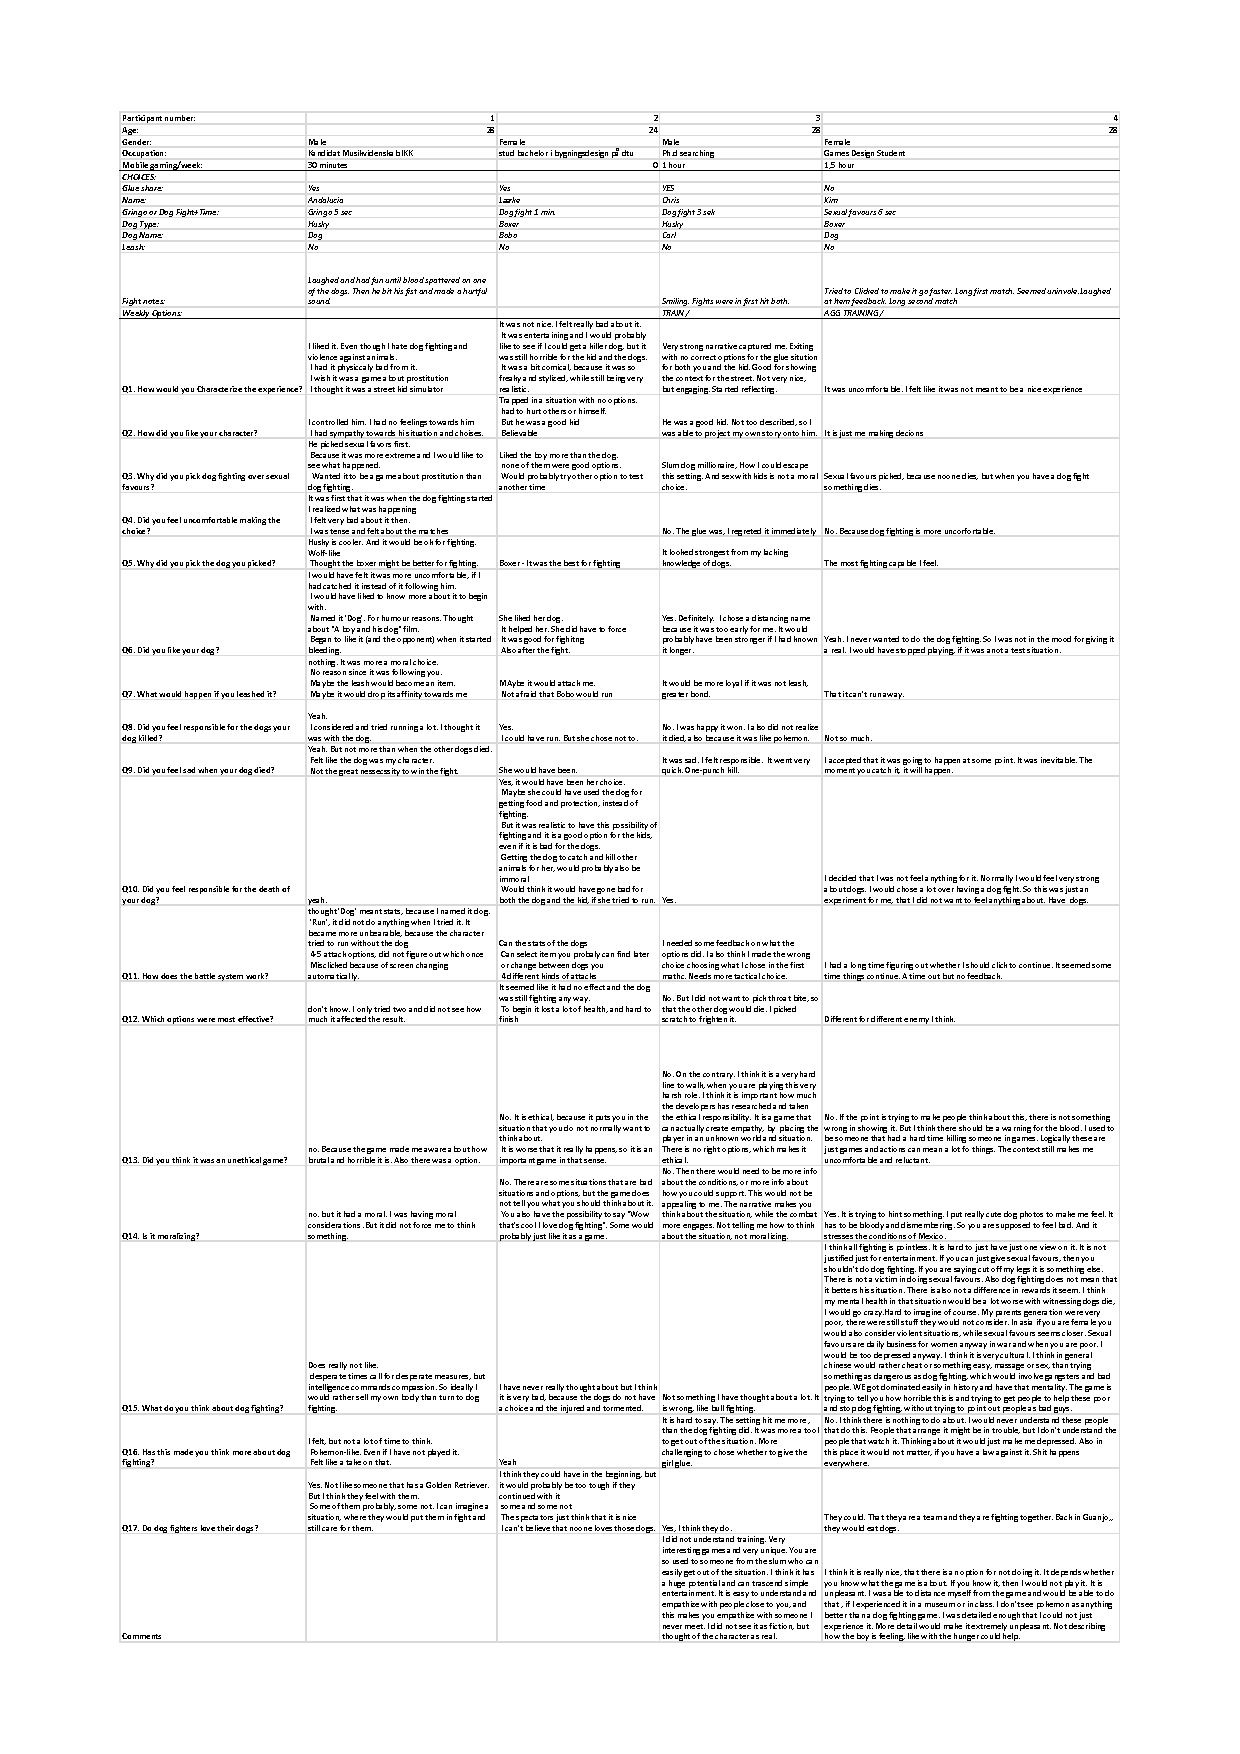
\includepdf[pages=-]{TestDataSheet1-2.pdf}

\end{document}

%%
%% End of file `elsarticle-template-1-num.tex'.